\documentclass{beamer}
\usepackage[utf8]{inputenc}
\usepackage{tikz}
\usepackage[]{algorithm2e}
\usetikzlibrary{arrows,matrix,positioning,quotes,shapes,graphs,automata}

\tikzset{
file_box/.style={
	% The shape:
	rectangle,
	% The size:
	minimum size=6mm,
	% The border:
	very thick,
	draw=red!50!black!50,
	% 50% red and 50% black,
	% and that mixed with 50% white
	% The filling:
	top color=white,
	% a shading that is white at the top...
	bottom color=red!50!black!20,
	% and something else at the bottom
	% Font
	font=\itshape
}
}

\tikzset{
prog_box/.style={
	% The shape:
	rectangle,
	% The size:
	minimum size=6mm,
	% The border:
	very thick,
	draw=blue!50!black!50,
	% 50% red and 50% black,
	% and that mixed with 50% white
	% The filling:
	top color=white,
	% a shading that is white at the top...
	bottom color=blue!50!black!20,
	% and something else at the bottom
	% Font
	font=\tt
},
hv path/.style={to path={-| (\tikztotarget)}},
vh path/.style={to path={|- (\tikztotarget)}},
skip loop/.style={to path={-- ++(0,#1) -| (\tikztotarget)}},
graphs/every graph/.style={edges=rounded corners}
}

\mode<presentation>
\usefonttheme{serif}

\definecolor{lightred}{rgb}{0.8,0.8,1}
\definecolor{lightgrey}{rgb}{0.8,0.8,0.8}


\title{CoRNG}
\author{Martin \textsc{Vassor}}
\institute{EPFL}
\beamertemplatenavigationsymbolsempty
\setbeamertemplate{footline}[frame number]

\date{November 10, 2016}
\begin{document}

\begin{frame}
	\titlepage
\end{frame}

\begin{frame}
	\frametitle{Introduction}
	\begin{itemize}
		\item K. \textsc{Antoniadis}, P. \textsc{Blanchard}, R. \textsc{Guerraoui} and J. \textsc{Stainer} (\textsc{lpd} -- \textsc{epfl}), 2016
		\item Benefits from lack of locality ?
	\end{itemize}
\end{frame}

\begin{frame}
	\frametitle{\textsc{CoRNG} overview}
	\begin{center}
		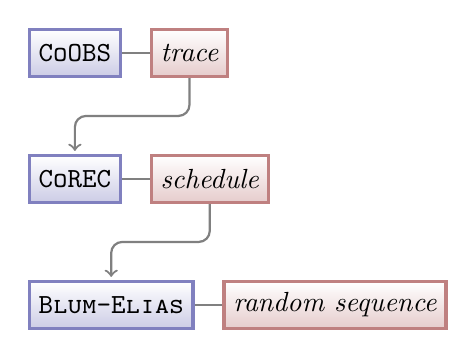
\begin{tikzpicture}[
				thick, black!50, text=black,
				every new ->/.style={shorten >=1pt},
			]
			\graph[grow right sep,
				branch down=16mm,
				simple
			]{
				"\textsc{CoOBS}"[prog_box] --
				tr/trace[file_box];
				tr -> [skip loop=-8mm]
				"\textsc{CoREC}"[prog_box] --
				sch/schedule[file_box];
				sch -> [skip loop=-8mm]
				"\textsc{Blum-Elias}"[prog_box] --
				random sequence[file_box];
			};
		\end{tikzpicture}
	\end{center}
\end{frame}

\begin{frame}[fragile]
	\frametitle{CoOBS}
	\begin{center}
		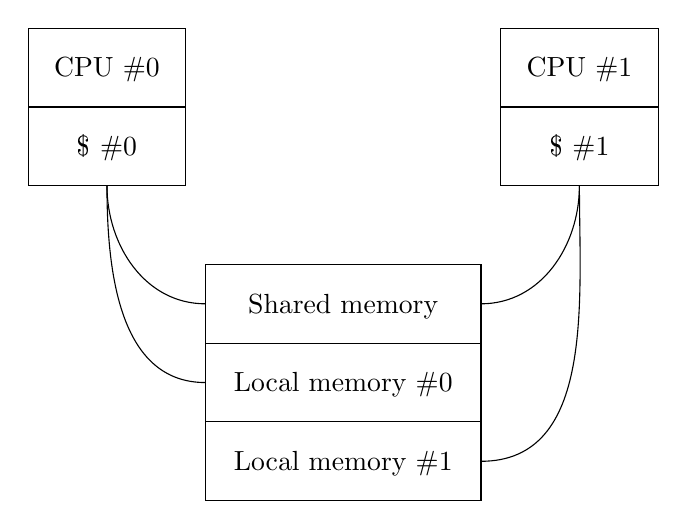
\begin{tikzpicture}[text height = 2.0ex]
			\draw (2, 3) rectangle (4,4) node [pos=.5] {CPU \#1};
			\draw (2, 2) rectangle (4,3) node [pos=.5] {\$ \#1};

			\draw (-2, 3) rectangle (-4,4) node [pos=.5] {CPU \#0};
			\draw (-2, 2) rectangle (-4,3) node [pos=.5] {\$ \#0};

			\draw (-1.75, 0) rectangle (1.75,1) node [pos=.5] {Shared memory};
			\draw (-1.75, -1) rectangle (1.75,0) node [pos=.5] {Local memory \#0};
			\draw (-1.75, -2) rectangle (1.75,-1) node [pos=.5] {Local memory \#1};

			\draw (3, 2) to [in=0, out=270] (1.75, .5);
			\draw (3, 2) to [in=0, out=270] (1.75, -1.5);

			\draw (-3, 2) to [in=180, out=270] (-1.75, .5);
			\draw (-3, 2) to [in=180, out=270] (-1.75, -.5);
		\end{tikzpicture}
	\end{center}
\end{frame}

\begin{frame}
	\frametitle{CoREC and \textsc{Blum-Elias}}
	\begin{description}
		\item [CoREC:] Rebuild schedule from local memories.
		\item [\textsc{Blum-Elias}:] Generate unbiased random from schedule.
	\end{description}
\end{frame}

\begin{frame}
	\frametitle{From schedule to unbiased randomness}
	\centering
		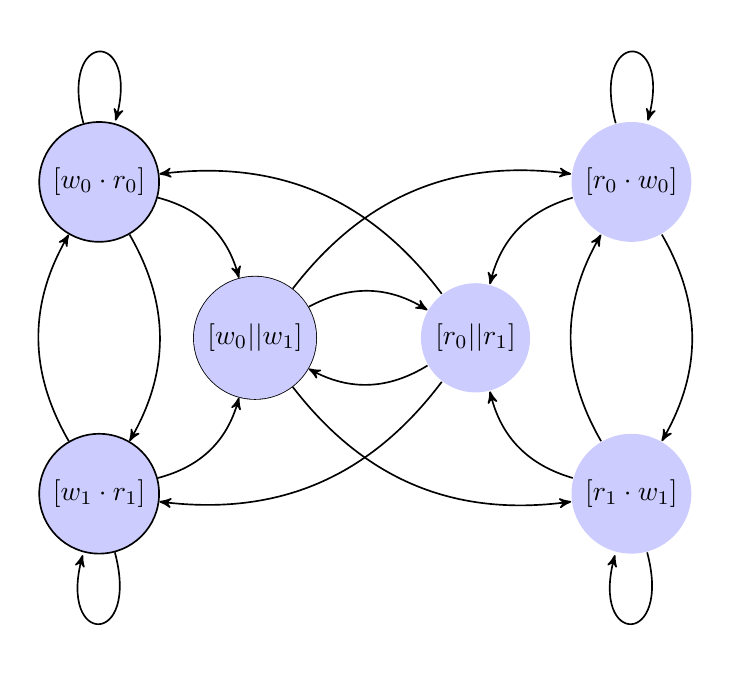
\begin{tikzpicture}[->,>=stealth',auto,node distance=2.8cm,semithick]
			\tikzstyle{every state}=[fill=lightred,draw=none,text=black]
			\node[state,draw=black] (ww) {$[w_0||w_1]$};
			\node[state,draw=black] (wr0)[above left of=ww] {$[w_0\cdot r_0]$};
			\node[state,draw=black] (wr1)[below left of=ww] {$[w_1\cdot r_1]$};
			\node[state] (ww) {$[w_0||w_1]$};
			\node[state] (rr)[right of=ww] {$[r_0||r_1]$};
			\node[state] (rw0)[above right of=rr] {$[r_0\cdot w_0]$};
			\node[state] (rw1)[below right of=rr] {$[r_1\cdot w_1]$};

			\path	(wr0) edge[bend left] (wr1)
				(wr0) edge[bend left] (ww)
				(wr0) edge[loop above] (wr0)
				(wr1) edge[bend left] (wr0)
				(wr1) edge[bend right] (ww)
				(wr1) edge[loop below] (wr1)
				(ww)  edge[bend left] (rw0)
				(ww)  edge[bend right] (rw1)
				(ww)  edge[bend left] (rr)
				(rr)  edge[bend right] (wr0)
				(rr)  edge[bend left] (wr1)
				(rr)  edge[bend left] (ww)
				(rw0) edge[bend left] (rw1)
				(rw0) edge[bend right] (rr)
				(rw0) edge[loop above] (rw0)
				(rw1) edge[bend left] (rw0)
				(rw1) edge[bend left] (rr)
				(rw1) edge[loop below] (rw1);
		\end{tikzpicture}
\end{frame}

\begin{frame}
	\frametitle{Conclusion}
	\begin{itemize}
		\item Requires data races.
		\item Uses order of atomic accesses.
		\item Better if more interleaving.
		\item Orders of magnitude faster\footnote{than current \texttt{/dev/random} for same quality}.
	\end{itemize}
\end{frame}

\begin{frame}
	\frametitle{References}
	\begin{itemize}
		\item Submitted to \emph{Distributed Computing} journal
	\end{itemize}
	\nocite{*}
	\bibliographystyle{plain}
	\bibliography{refs} 
\end{frame}

\end{document}
